% This file contains the content for the Results section

In this section the transient performance test results for the scheduled and controlled FVAN will be presented. Attention will be given to thrust lapses and fan stall margin. If the FVAN actuator turns out to be slow, time constant value will be decremented in steps to determine how fast the actuator must be for acceptable performance.

An NPSS model developed for a conventional high BPR turbofan in the SSA thrust class was linked with TTECTrA in Matlab Simulink through an S-function. The results for the controller development are presented here to illustrate how the work proposed in this paper will be shown.

The set points for the conventional high BPR turbofan are given in \autoref{fig:set_points}. The set point variables are $EPR$, $N_f$, $N_c$, and $Wf$ whereas the set point function is for net thrust. The set point functions are not exactly linear but they can be approximated with linear relations if necessary.  

% Set points figure
\begin{figure}[!htb]
    \begin{center}
    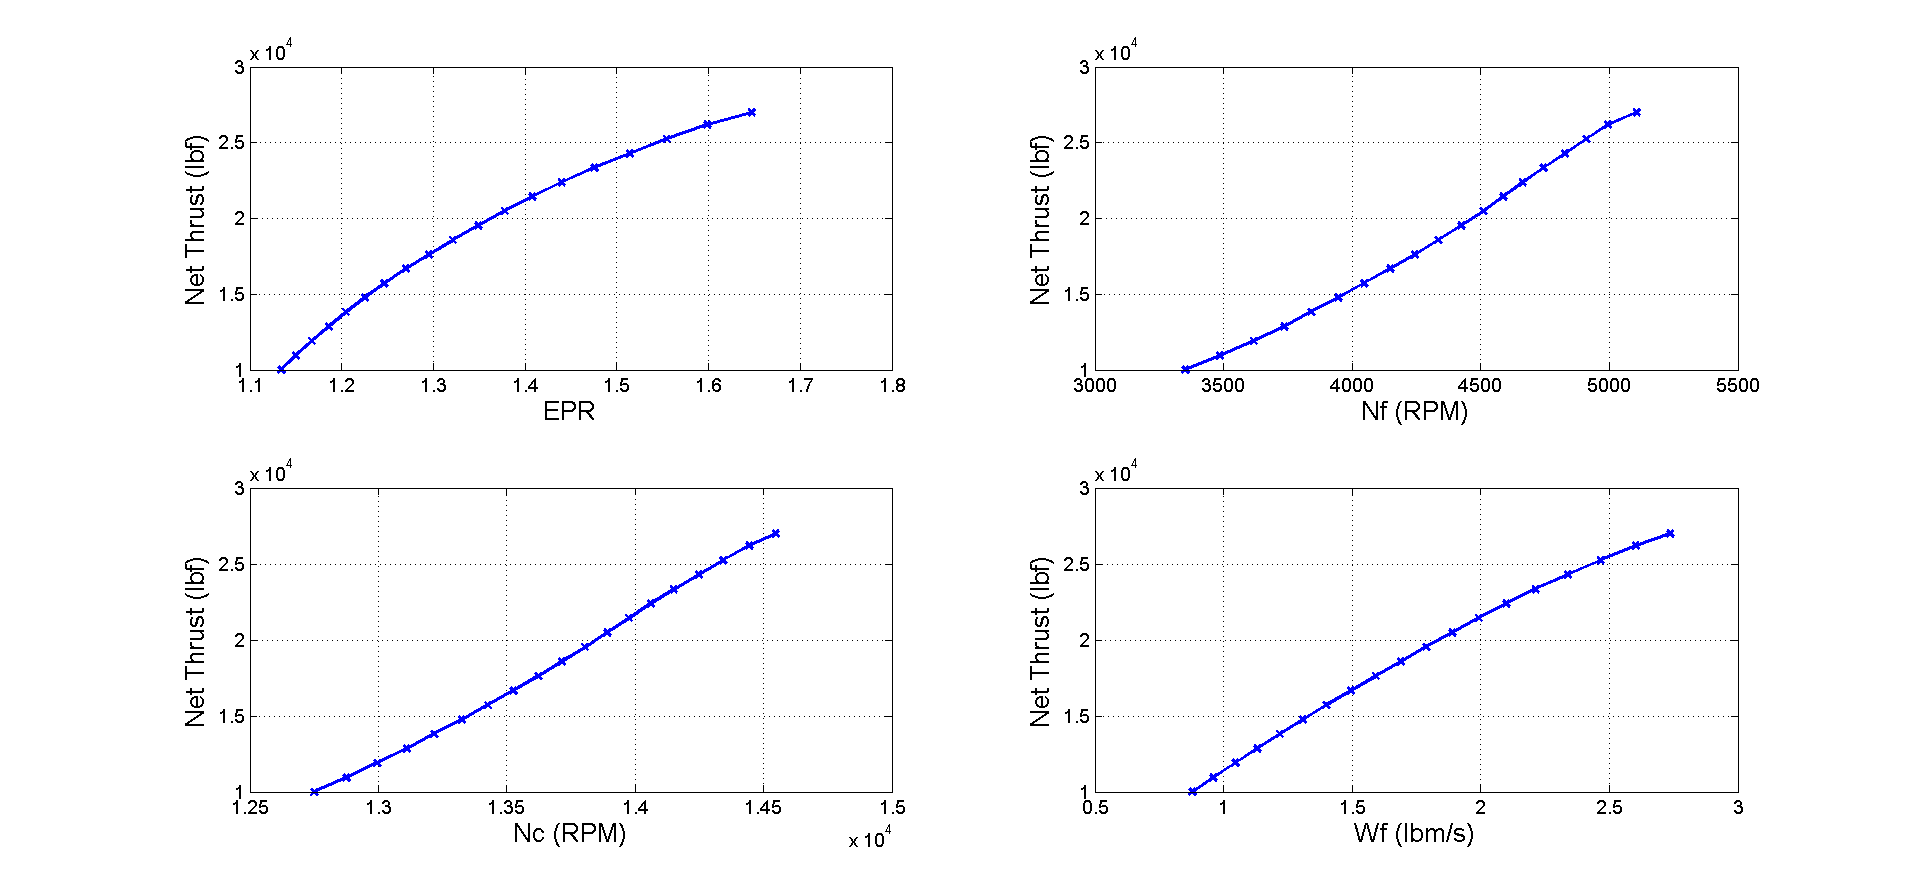
\includegraphics[width=\textwidth, height=\textheight,keepaspectratio]{set_points.png}
    \caption{Set points for the conventional high BPR turbofan}
    \label{fig:set_points}
    \end{center}
\end{figure}

\autoref{fig:acceleration_schedule} presents the acceleration schedule for the conventional high BPR turbofan. This schedule is used in the limiter for acceleration. The schedule was determined by running more and more demanding signals until the HPC stall margin limit was reached. 

% Acceleration schedule figure
\begin{figure}[!htb]
    \begin{center}
    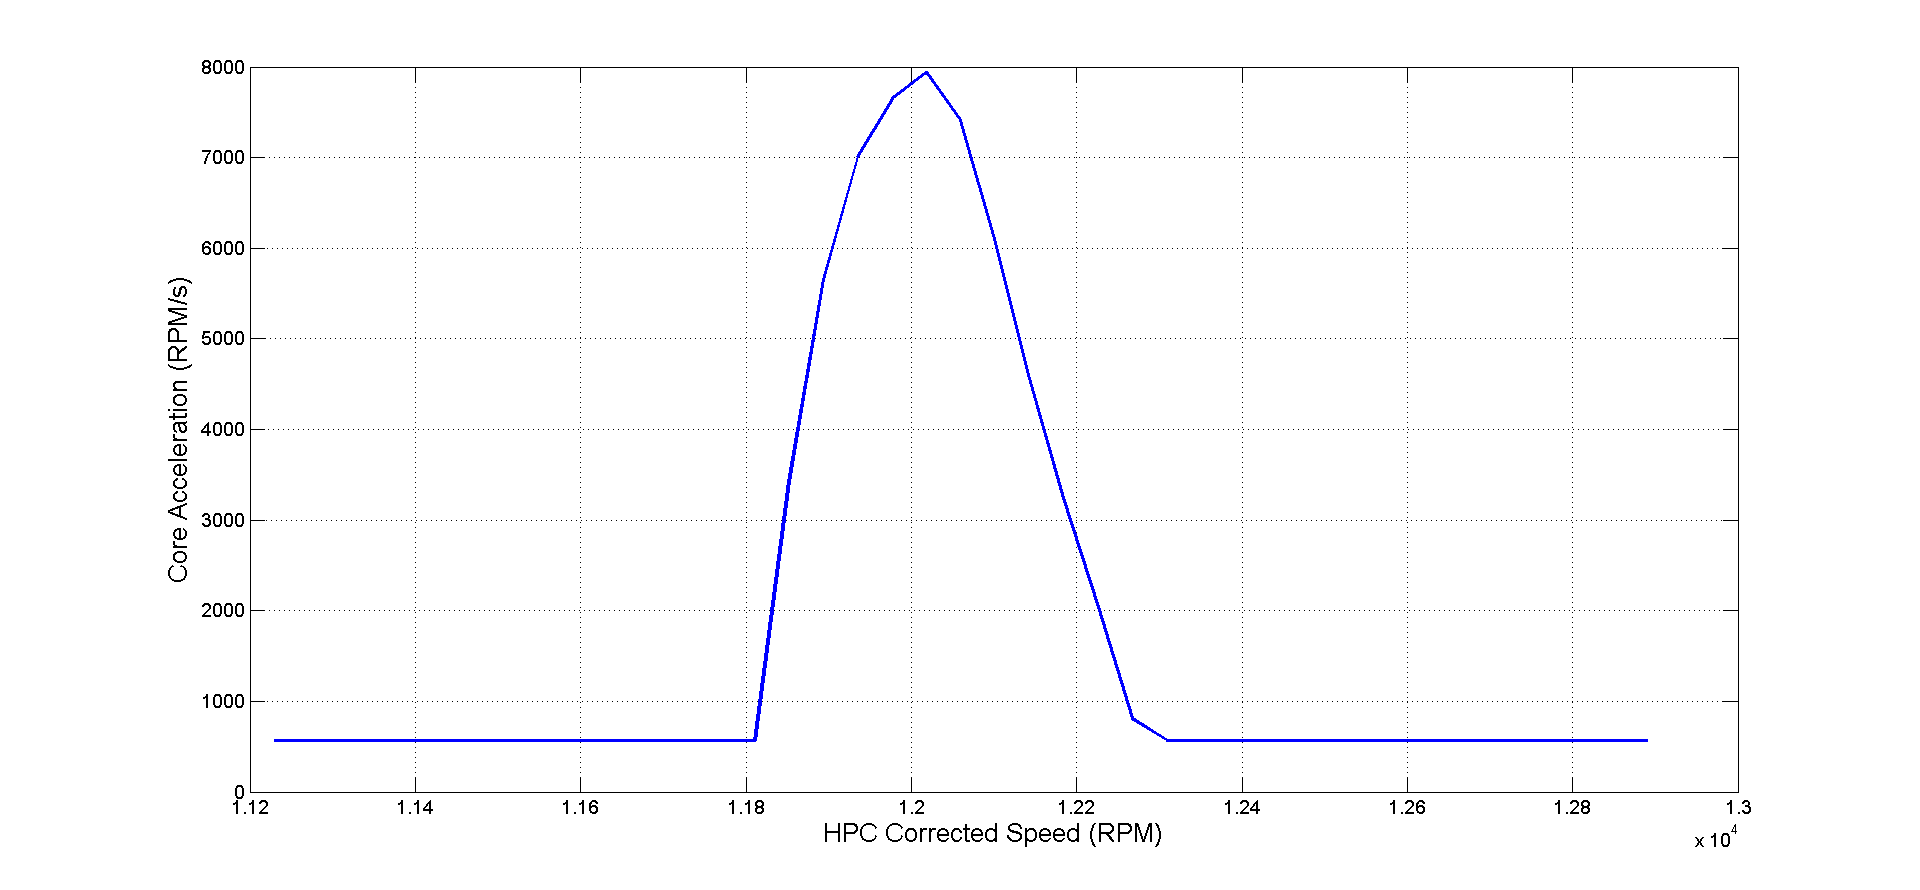
\includegraphics[width=\textwidth, height=\textheight,keepaspectratio]{acceleration_schedule.png}
    \caption{Acceleration schedule for the conventional high BPR turbofan}
    \label{fig:acceleration_schedule}
    \end{center}
\end{figure}

The conventional high BPR turbofan net thrust response for a signal with a series of steps, chops, and ramps is in \autoref{fig:net_thrust_response}. The controller follows the demand in an acceptable manner.

% Net thrust response figure
\begin{figure}[!htb]
    \begin{center}
    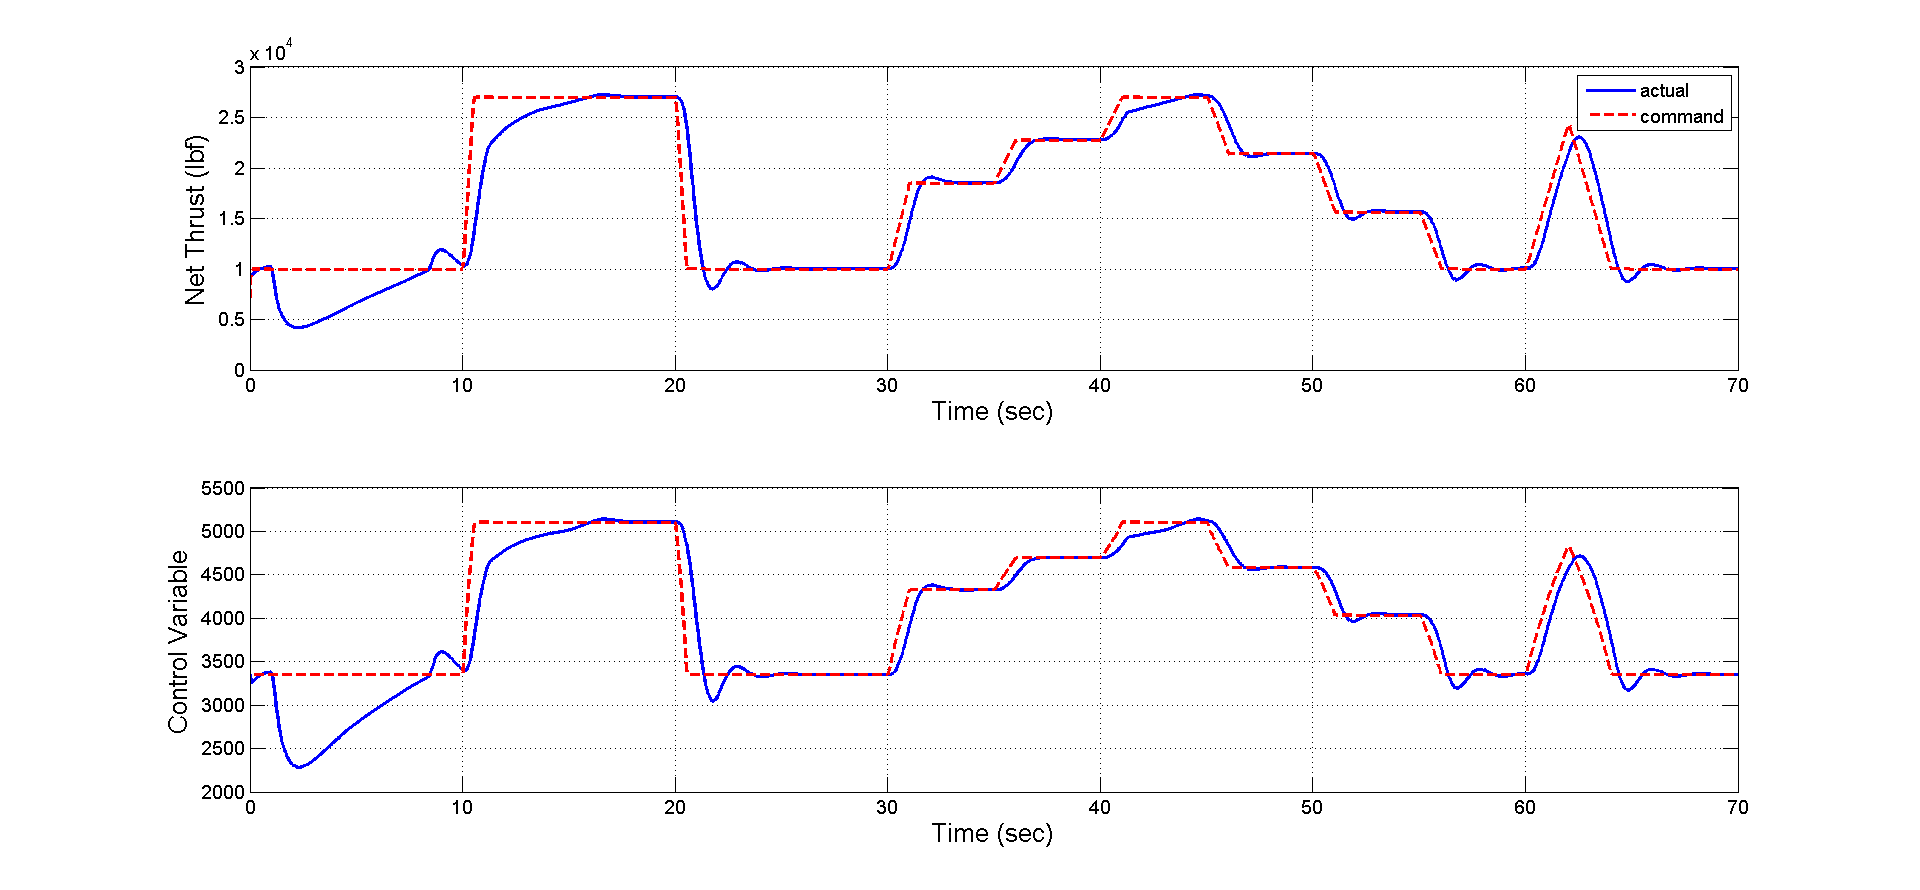
\includegraphics[width=\textwidth, height=\textheight,keepaspectratio]{net_thrust_response.png}
    \caption{Conventional high BPR turbofan net thrust response}
    \label{fig:net_thrust_response}
    \end{center}
\end{figure}

How the HPC surge margin changes throughout the net thrust response is shown in \autoref{fig:HPC_surge_margin}. The HPC stall margin did not come close to the limit throughout the entire transient. Also, \autoref{fig:HPC_surge_margin} gives the core acceleration against the acceleration schedule during the transient. The largest core acceleration recorded throughout the transient is less than a quarter of the maximum in the acceleration schedule. 

% HPC surge margin figure
\begin{figure}[!htb]
    \begin{center}
    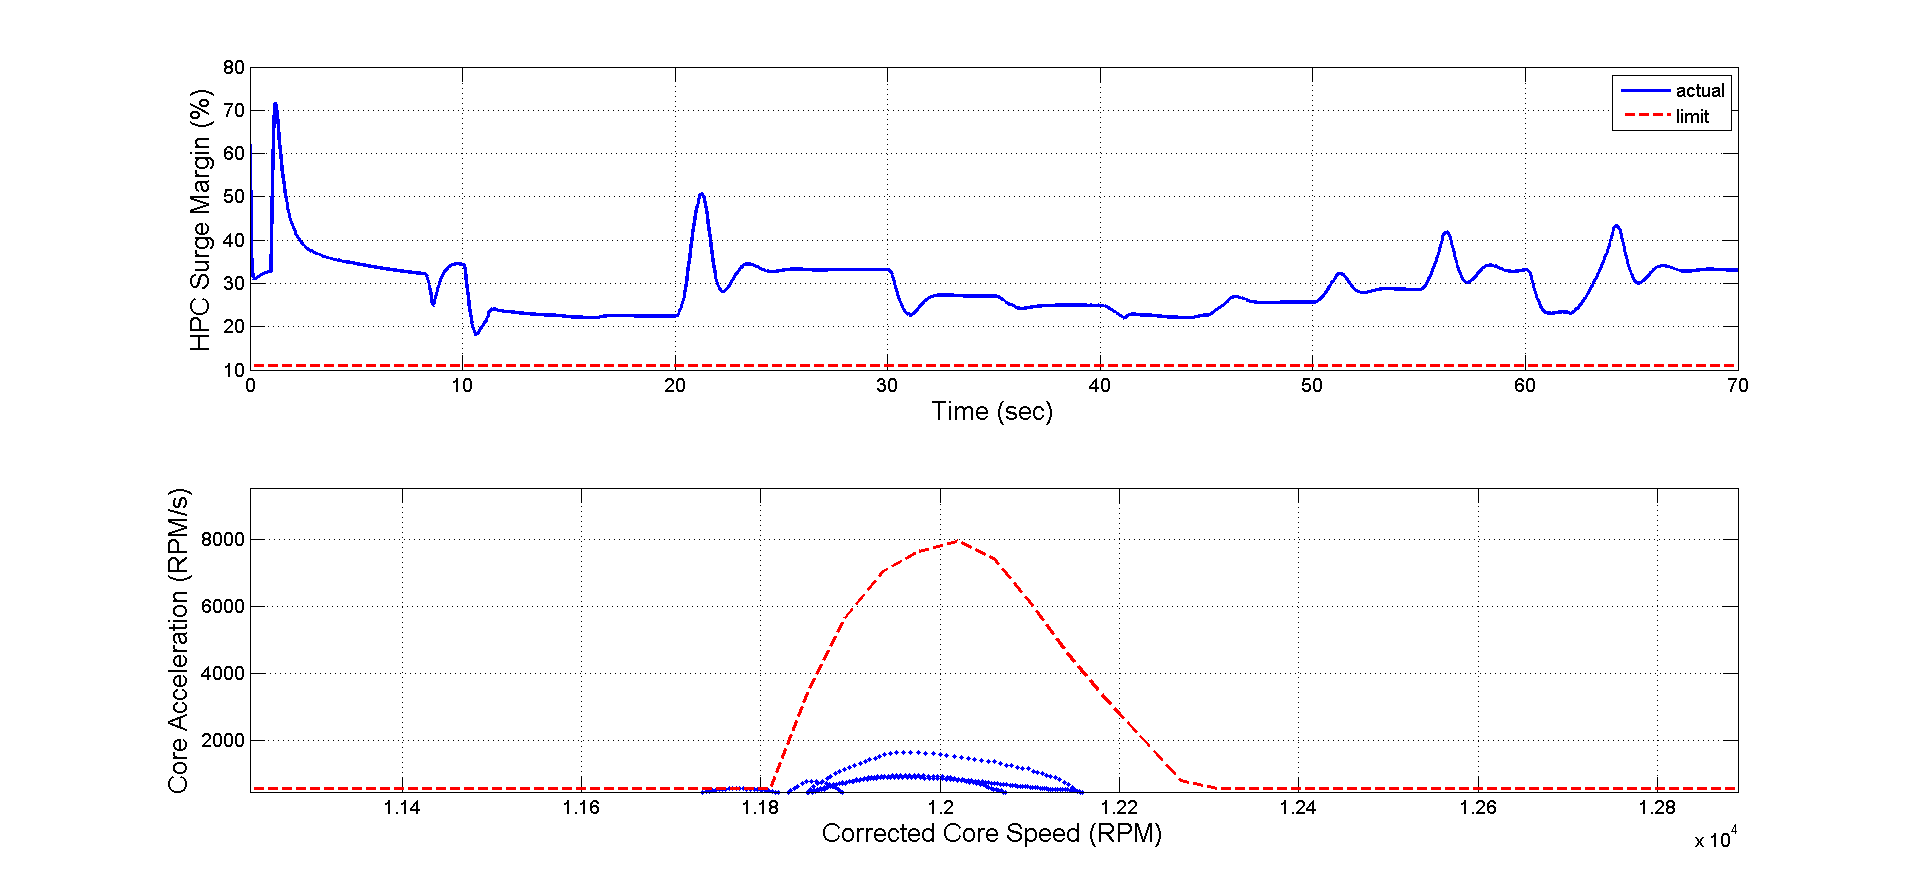
\includegraphics[width=\textwidth, height=\textheight,keepaspectratio]{HPC_surge_margin.png}
    \caption{Conventional high BPR turbofan HPC surge margin response}
    \label{fig:HPC_surge_margin}
    \end{center}
\end{figure}

Similar to the HPC case, \autoref{fig:LPC_surge_margin} shows how the LPC surge margin changed throughout the transient. The controller maintained the LPC stall margin more than 10\% during transient. \autoref{fig:LPC_surge_margin} also shows the change in combustor loading, $W_f/P_{s3}$, to measure combustor stability throughout the entire transient. The controller managed to keep the combustor loading above the limit in addition to the HPC and LPC stall margins.

% LPC surge margin figure
\begin{figure}[!htb]
    \begin{center}
    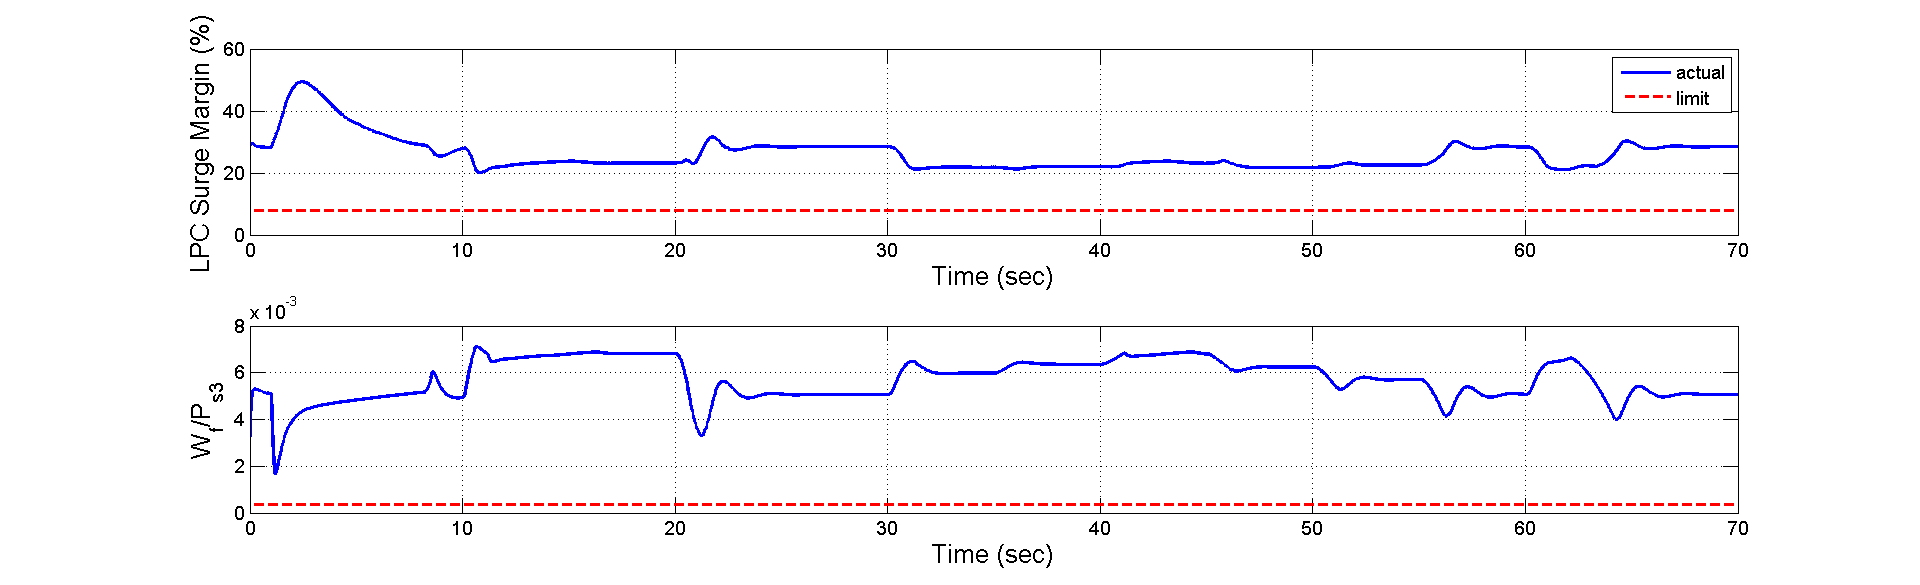
\includegraphics[width=\textwidth, height=\textheight,keepaspectratio]{LPC_surge_margin.png}
    \caption{Conventional high BPR turbofan LPC surge margin response}
    \label{fig:LPC_surge_margin}
    \end{center}
\end{figure}